\documentclass{article}

% Language setting
% Replace `english' with e.g. `spanish' to change the document language
\usepackage[english]{babel}

% Set page size and margins
% Replace `letterpaper' with `a4paper' for UK/EU standard size
\usepackage[letterpaper,top=2cm,bottom=2cm,left=3cm,right=3cm,marginparwidth=1.75cm]{geometry}

% Useful packages
\usepackage{amsmath}
\usepackage{graphicx}
\usepackage{listings}
\usepackage{xspace}
\usepackage{booktabs}
\usepackage{paralist}
\usepackage{stfloats}
\usepackage{float}
\usepackage{enumitem}
\usepackage{etaremune}

\usepackage{subcaption}

\newcommand{\specialcell}[2][c]{%
  \begin{tabular}[#1]{@{}l@{}}#2\end{tabular}}
 
\usepackage[colorlinks=true, allcolors=blue]{hyperref}

\title{Experiment Setting Details}
% \author{You}
\date{}

\begin{document}
\maketitle

% \section{Experiment Setting}


% We have discussed capabilities' broad applications for ML engineering across different stages, stakeholders, and attributes.
% However, there still exist many challenges in integrating capabilities into ML engineering. 
% We next list challenges and discuss their research opportunities.


\paragraph{Data}
We use the \textsc{Amazon-wilds} dataset~\cite{pmlr-v139-WILDS} for sentiment analysis.
The dataset consists of Amazon reviews of many different categories and their ratings.
We select \textsc{Home-and-kitchen} category for training and 10 other categories for evaluation. 
In domain adaptation, the \textsc{Home-and-kitchen} category would be referred to as source domain, while other categories are target domains. 
Following previous work in domain adaptation~\cite{blitzer-etal-2007-biographies}, we convert ratings to binary labels (positive when >3, negative when <3) and sample a balanced dataset for each category (domain).

\paragraph{Model}
% We select two model architectures for our evaluation: LSTM and BERT~\cite{bhargava2021generalization, DBLP:journals/corr/abs-1908-08962}.
% We trained 200 LSTM models and 
To obtain a series of models with different accuracies, we finetuned a pre-trained BERT model~\cite{bhargava2021generalization, DBLP:journals/corr/abs-1908-08962} 100 times on different random seeds.



\begin{table}[h]
\centering
\begin{tabular}{l p{0.8\linewidth}}
\toprule
\textbf{Capability} & \textbf{Keywords} \\
\midrule 
negation   &  not, n't \\
\specialcell[t]{negation \\\emph{(variant)}} & no, never, neither, nobody, none, nor, nothing \\
shifter & refuse, reject, deny, doubt, abandon, miss, question, abort, stop \\
modality & would have, could have, should have \\
comparative & better, worse, than \\
mixed & but, however, though, although, despite, even if, rather than, except that \\
reducer & kind of, all that, less, a little, somewhat, still \\
amplifier & really, very, super, so, incredibly, extremely, at all, whatsoever, much \\
\bottomrule
\end{tabular}

\caption{Capabilities and their instantitation keywords for sentiment analysis, selected based on existing work~\cite{barnes-etal-2019-sentiment}. We slice the validation data on keywords to instantiate these capabilities.
}
\label{tab:cap-inst}
\end{table}

\paragraph{Method}


Our goal is to observe the correlations between models' accuracies across source domain and target domains,
as well as how extra information (e.g., accuracies on capability test suites) would affect the correlations.

We first use a linear model to compute the correlations of accuracies between source domain and target domains, without any extra variables.
We then introduce three sets of variables to the linear model:

\begin{enumerate}
    \item \textit{Capability test suites' accuracies}: we first selected 8 capabilities for sentiment analysis based on an existing study~\cite{barnes-etal-2019-sentiment}. We instantiated these capabilities by slicing the source domain dataset on their corresponding keywords (see Tab.~\ref{tab:cap-inst}).
    The final capabilities we used are \textit{shifter}, \textit{modality}, and \textit{comparative}.
    \item \textit{Random subsets' accuracies}: we selected three random subsets from source dataset. These subsets are of the same size of three capability test suites. We computed models' accuracies on the random subsets.
    \item \textit{Noisy accuracies}:  we added random Gaussian noise to models' validation accuracies.
    % \item \textit{Long text subset's accuracies}: we selected texts longer than 150 tokens from source dataset and computed models' accuracies on the slice.
\end{enumerate}

For the last two settings, we repeat the process on 100 different random seeds and average their results.

We then fit the linear model with these extra variables for each setting.
We looked at adjusted $R^2$ to see whether the model has a better fit (i.e., whether these extra variables help predict out-of-distribution scores). 
\footnote{$R^2$ represents the proportion of the variance that could be explained by input variables. 
Higher $R^2$ implies a better fit of the linear model and higher predictive power of input variables.
We used adjusted $R^2$ to compensate the effect of extra degrees of freedom. It only increases if the new variable enhances the model above what would be obtained by chance.}
We also performed \textsc{ANOVA} testing to see whether the improvement is statistically significant. 

To understand the relation between capabilities' predictiveness and distribution distance, we followed the method from previous work~\cite{blitzer-etal-2007-biographies} to compute a proxy $\mathcal{A}$-distance between different domains.

% \section{Experiment Results}
% We found that capabilities better help predict model generalization compared to all other baselines.
% The linear model's adjusted $R^2$ increases (statistically significantly) in 50\% domains with extra variables from capabilities.
% In contrast, the best baseline (random subsets) only increases adjusted $R^2$ in 20\% domains on average (see Fig.~\ref{fig:improvement} for details).

% For finetuned BERT models, that adjustd $R^2$ increases significantly in 5 out of 10 casese

% We found that different capabilities add different information for prediction.
% Some capabilities (e.g., \textit{negation}) produce too many test cases, which leads to an uninformative distribution close to the original dataset.
% Different capabilities could also augment each other: 
% \textit{shifter} improves predictive power in 2 cases, but adding \textit{modality} further increases predictive power in 4 cases.


% We found that capabilities' predictiveness correlates with distribution distance (see Fig.~\ref{fig:distance}). 
% The further the domain is, the better capabilities could help predict generalization.
% We hypothesize that this might be due to the fact that if a target domain is too close to the source domain,
% there is little room left for improvement.




% \begin{figure}[h]
%     \centering
%     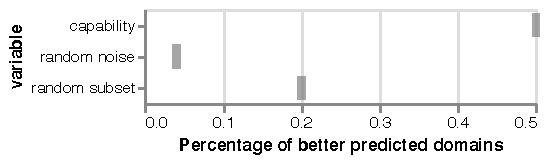
\includegraphics[width=0.5\linewidth]{figures/plot-improvement}
%     \vspace{-10pt}
%     \caption{Capabilities better help predict model generalization compared to other baselines.}
%     \label{fig:improvement}
% \end{figure}



% \begin{figure}[t]
% \begin{subfigure}[b]{0.5\linewidth}
%   \centering
%   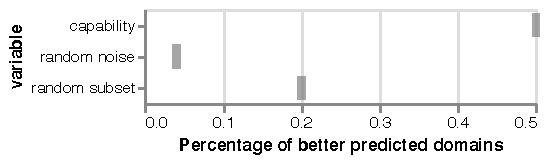
\includegraphics[width=0.8\linewidth]{figures/plot-improvement}
% \vspace{-10pt}
% \caption{Capabilities better help predict model generalization compared to other baselines.}
%   \label{fig:rel-data:b}
% \end{subfigure}
% \begin{subfigure}[b]{0.5\linewidth}
%   \centering
%  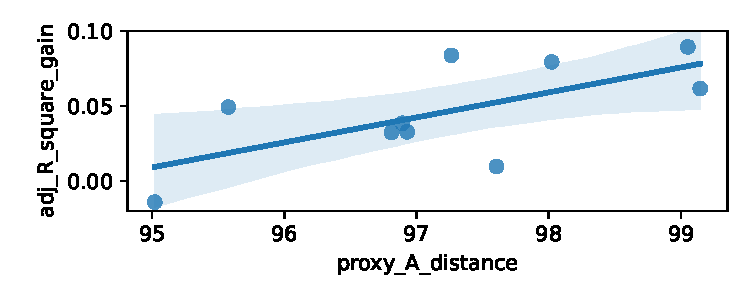
\includegraphics[width=0.8\linewidth]{figures/plot-distance.pdf}
%     \caption{Predictiveness improvement correlates with distribution distance.
%     The further the distribution is, the better capabilities could help predict generalization. 
%     We hypothesize that this is because if a target distribution is too close to the source distribution, there is little room left for improvement.
%     }
%   \label{fig:rel-data:a}
% \end{subfigure}
%   \label{fig:rel-data}
% \end{figure}

% \begin{figure}[h]
%     \centering
%     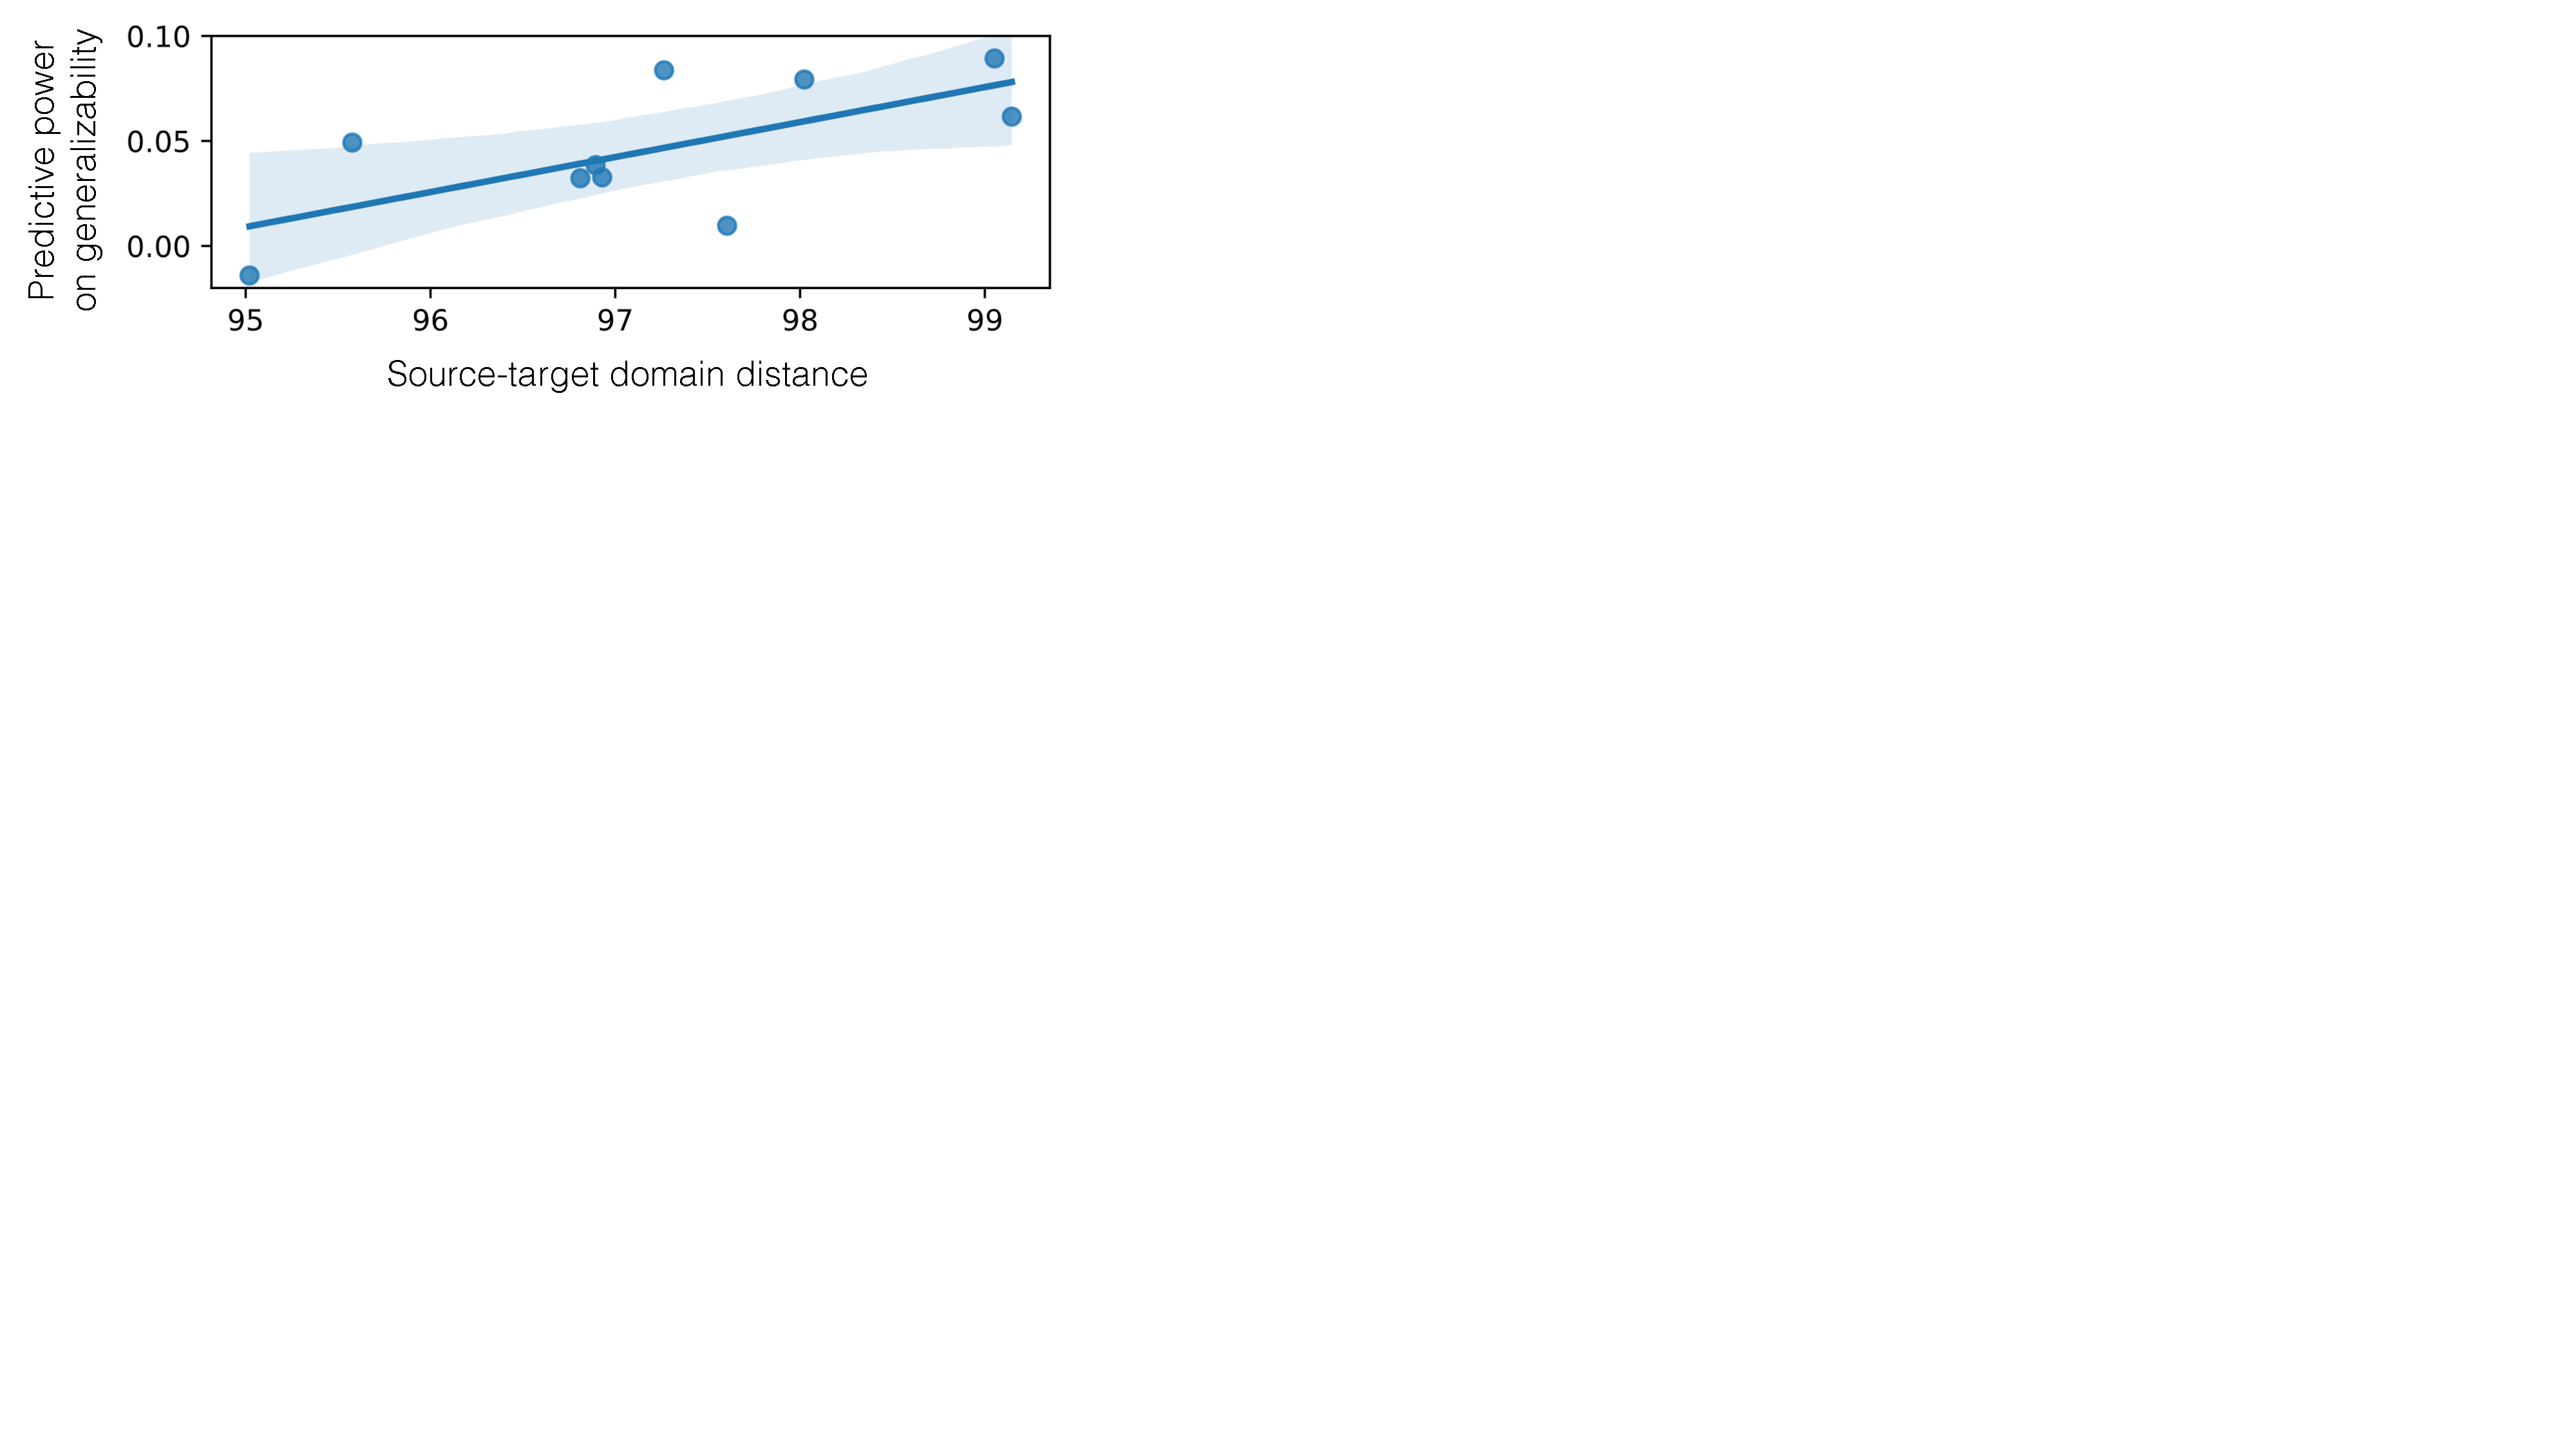
\includegraphics[trim={0cm 27cm 40cm 0cm}, clip,width=0.6\linewidth]{figures/plot-distance-v2.pdf}
%     \caption{Predictiveness improvement correlates with distribution distance.
%     The further the distribution is, the better capabilities could help predict generalization. 
%     We hypothesize that this is because if a target distribution is too close to the source distribution, there is little room left for improvement.
%     }
%     \label{fig:distance}
% \end{figure}


\bibliographystyle{acm}
\bibliography{sample}

\end{document}